\documentclass[11pt,a4paper]{article}
\usepackage[margin=2.2cm]{geometry}
\usepackage[T1]{fontenc}
\usepackage[utf8]{inputenc}
\usepackage{lmodern}
\usepackage{booktabs}
\usepackage{graphicx}
\usepackage{subcaption}
\usepackage{amsmath}
\usepackage{float}
\usepackage{xcolor}
\usepackage[colorinlistoftodos,textsize=small]{todonotes}
\usepackage[hidelinks]{hyperref}

% ---------------------------------------------------------------------------
% Helpers: every table is generated by the code (report/tables/*.tex)
% ---------------------------------------------------------------------------
\newcommand{\inputtable}[1]{\IfFileExists{tables/#1.tex}{\input{tables/#1.tex}}{\fbox{\textbf{missing generated table: #1}}}}
\newcommand{\fig}[3][0.95]{%
  \begin{figure}[H]\centering
  \IfFileExists{figures/#2.pdf}{\includegraphics[width=#1\linewidth]{figures/#2.pdf}}{\fbox{missing figure #2}}
  \caption{#3}\label{fig:#2}\end{figure}}
\newcommand{\studenttodo}[1]{\todo[inline,color=orange!25]{\textbf{Student interpretation:} #1}}

\IfFileExists{tables/q1_macros.tex}{\newcommand{\NTotal}{45211}
\newcommand{\NTrain}{31647}
\newcommand{\NVal}{6782}
\newcommand{\NTest}{6782}
\newcommand{\PosRate}{0.1170}
}{}
\IfFileExists{tables/q3_macros.tex}{\newcommand{\RegNTrain}{14447}
\newcommand{\RegNVal}{3096}
\newcommand{\RegNTest}{3097}
}{}

\newcommand{\StudentName}{İhsan Yağız Sakızlıoğlu}
\newcommand{\StudentID}{300201071}
\newcommand{\RepoURL}{\url{https://github.com/ihsanyagiz/ceng463-take-home-mid}}

\title{CENG 463 -- Machine Learning\\Take-Home Midterm Report}
\author{\StudentName\ (\StudentID)\\ Repository: \RepoURL}
\date{\today}

\begin{document}
\maketitle
\listoftodos[Interpretation placeholders to be written by the student]
\tableofcontents
\clearpage

\section{Introduction, research questions, and datasets}
\label{sec:intro}

% TODO(student): interpret / motivate the study in your own words
\studenttodo{Motivation of the study and the research questions in your own words, e.g.:
(i) how much does a leakage-safe protocol change reported performance (Q1);
(ii) how do linear, probabilistic and instance-based classifiers compare on an imbalanced, mixed-type task (Q2);
(iii) how do complexity and regularisation affect regression generalisation (Q3);
(iv) what do tree ensembles add over single trees and the Q2 models (Q4);
(v) which model is defensible when performance, robustness, uncertainty and cost are all considered (Q5).}

\paragraph{Classification dataset (Q1, Q2, Q4, Q5).}
UCI Bank Marketing (\texttt{bank-full}, UCI id 222, \cite{moro2014bank}), loaded with \texttt{ucimlrepo} and cached in
\texttt{data/raw/}. Each row is one client contacted in a Portuguese bank's direct-marketing phone campaign; the
binary target \texttt{y} indicates whether the client subscribed to a term deposit. The table has \NTotal{} rows
and 16 predictors (7 integer, 9 categorical); the overall positive rate is \PosRate{}
(Table~\ref{tab:q1_class_dist}). Categorical values recorded as \texttt{"unknown"} are delivered as missing
values by \texttt{ucimlrepo}.

\paragraph{Regression dataset (Q3).}
California Housing \cite{pace1997sparse} via \texttt{sklearn.datasets.fetch\_california\_housing}: 20{,}640
census block groups, 8 numeric predictors, target \texttt{MedHouseVal} = median house value in units of
\$100{,}000 (capped at 5.0).

\section{Data audit, preprocessing, and leakage controls}
\label{sec:audit}

\subsection{Q1a: Dataset audit}
\inputtable{q1_audit}
\inputtable{q1_anomalies}
\inputtable{q1_class_dist}
\inputtable{q1_duration_by_target}
\fig{q1_numeric_distributions}{Distributions of heavy-tailed / sentinel-valued numeric features (log count axis).}

% TODO(student): interpret
\studenttodo{Q1a: describe domain, target, feature types; discuss missing/\texttt{unknown} values
(esp.\ \texttt{poutcome}, \texttt{contact}), duplicates, anomalies (\texttt{pdays}=-1 sentinel, negative
\texttt{balance}, \texttt{campaign} extremes) and why \texttt{duration} is a problematic (leaking) predictor.}

\subsection{Q1b: Partitioning}
A stratified 70/15/15 train/validation/test split was created once with seed 42 before any fitting
(Table~\ref{tab:q1_split_sizes}); indices are stored in \texttt{data/splits/}. Partition sizes:
train \NTrain, validation \NVal, test \NTest. Stratified and plain random splitting were each repeated over 100
seeds on the full data and on a random 200-row sample (Table~\ref{tab:q1_split_comparison},
Figure~\ref{fig:q1_split_deviation}).
\inputtable{q1_split_sizes}
\inputtable{q1_split_comparison}
\fig{q1_split_deviation}{Absolute deviation of the positive-class proportion of each partition from the reference proportion, over 100 seeds.}

% TODO(student): interpret
\studenttodo{Q1b: justify the 70/15/15 + CV design; compare stratified vs.\ random deviations (full vs.\
small sample: zero/few positives in val/test); when can stratification itself fail (e.g.\ very rare classes,
temporal/grouped data, distribution shift, multi-label)?}

\subsection{Q1c: Leakage-safe preprocessing}
All transformations are steps of an sklearn/imblearn \texttt{Pipeline} (\texttt{src/preprocessing.py}) and are
therefore fit only on the training data or on the training folds of cross-validation. Numeric features: median
imputation, then standardisation (LogReg, kNN, GaussianNB) or quantile discretisation (BernoulliNB) or no
scaling (trees). Categorical features: missing values mapped to an explicit \texttt{"missing"} level, then
one-hot encoding with \texttt{handle\_unknown="ignore"} (unseen categories become an all-zero vector). The only
row-wise engineering (no fitted statistics) is the indicator \texttt{prev\_contacted} = [\texttt{pdays} $\neq -1$].
\inputtable{q1_transform_matrix}

% TODO(student): interpret
\studenttodo{Q1c: explain why each transformation matters (or not) for each model family (scale sensitivity of
distances/penalties, NB distributional assumptions, split invariance of trees); justify the constant
\texttt{"missing"} level instead of most-frequent imputation.}

\subsection{Q1d: Controlled leakage demonstration}
Model: Logistic Regression ($C=1$, \texttt{class\_weight=balanced}). Rows labelled \textbf{INVALID} are
deliberately wrong and are used only for this demonstration: INVALID\_1 includes \texttt{duration};
INVALID\_2 fits scaling and \texttt{SelectKBest}(k=20) on all development rows (train+validation) before CV;
INVALID\_3 adds the mean target of a high-cardinality group (job $\times$ month $\times$ day) computed on all
development rows including the row itself. The corresponding valid procedures fit the same steps inside the
pipeline (for target encoding, sklearn's cross-fitted \texttt{TargetEncoder}). The test set is not used.
\inputtable{q1_leakage_demo}
\fig{q1_leakage_demo}{Cross-validation and validation Macro-F1 of valid vs.\ deliberately INVALID procedures.}

% TODO(student): interpret
\studenttodo{Q1d: quantify the apparent improvement of each INVALID procedure over its valid counterpart and
explain why it is untrustworthy (information unavailable at prediction time / information from evaluation rows
entering the fit). Note which leakage was large and which was small here and why (e.g.\ global scaling with
31k rows changes little; target encoding of rare groups memorises labels).}

\subsection{Q1e: Protocol diagram and failure modes}
\fig{q1_protocol}{Experimental protocol.}

% TODO(student): interpret
\studenttodo{Q1e: explain at least three failure modes that invalidate results even if the code runs (e.g.\
preprocessing fit outside folds, selecting on test, leaking post-outcome features, duplicate/near-duplicate
rows across partitions, temporal ordering of campaigns, threshold tuned on evaluation data, unstable single
split / no variance estimate).}

\section{Methods and experimental design (Questions 1--5)}
\label{sec:methods}

\paragraph{Q1.} Audit on all rows (descriptive only); split once; leakage demonstration with LogReg (Section~\ref{sec:audit}).

\paragraph{Q2 (\texttt{src/q2\_classifiers.py}).} Majority-class \texttt{DummyClassifier}, Logistic Regression
(L2, lbfgs), Naive Bayes and $k$-NN. For Naive Bayes two representations were compared under the same CV:
GaussianNB on standardised numeric + one-hot features, and BernoulliNB on quantile-binned (one-hot) numeric +
one-hot categorical features; the representation with the higher CV Macro-F1 was retained. Imbalance study
(Q2d): with all other hyper-parameters fixed, LogReg without intervention vs.\ \texttt{class\_weight=balanced}
vs.\ training-only \texttt{RandomOverSampler} vs.\ training-only SMOTE (inside \texttt{imblearn.Pipeline}), and
$k$-NN with/without oversampling. A decision-threshold sweep for the finalised Q2 model selects the threshold
on out-of-fold training predictions and only reports it on validation. Error analysis (Q2e) exports the 10 most
confident false negatives and 10 most confident false positives on validation.

\paragraph{Q3 (\texttt{src/q3\_regression.py}).} Separate random 70/15/15 split (seed 42; \RegNTrain/\RegNVal/\RegNTest).
DummyRegressor (mean), OLS, Ridge, Lasso, DecisionTreeRegressor and RandomForestRegressor, all with
\texttt{StandardScaler} inside the pipeline. Complexity curves: polynomial degree 1--4 (Ridge, $\alpha=10^{-3}$)
and tree depth 1--20, training vs.\ 5-fold CV RMSE; learning curves for OLS and an unpruned tree. Ridge/Lasso
$\alpha$ chosen by 5-fold CV RMSE; coefficient paths, sparsity and bootstrap stability of coefficients of
correlated predictors.

\paragraph{Q4 (\texttt{src/q4\_trees\_ensembles.py}).} Decision Tree, Random Forest, AdaBoost (decision stumps,
SAMME) and Gradient Boosting (depth-3 trees), plus the best Q2 model as reference, with the same split and CV.
Boosting is tuned with \emph{staged} 5-fold CV: for each learning rate and sample-weighting option one model with
the maximum number of estimators is fit per fold and evaluated at every checkpoint of
\texttt{n\_estimators} (equivalent to a grid over \texttt{n\_estimators}). Random-Forest tree correlation is
measured as the mean pairwise Pearson correlation of per-tree $P(\text{yes})$ on validation. Importances:
impurity-based (one-hot columns summed back to the original feature) vs.\ permutation importance on validation
(5 repeats, $\Delta$Macro-F1); a control experiment adds pure-noise features and a near-duplicate of
\texttt{age}.

\paragraph{Q5 (\texttt{src/q5\_robustness\_selection.py}, \texttt{src/q5\_final\_test.py}).} Seven frozen candidates
(LogReg, NaiveBayes, kNN, DecisionTree, RandomForest, AdaBoost, GradientBoosting). Repeated stratified CV
(5 folds $\times$ 3 repeats). Robustness on validation: (i) Gaussian noise added to the six continuous features
with SD = severity $\times$ training SD, severities $\{0, 0.1, 0.25, 0.5, 1.0\}$; (ii) a fraction
$\{0, 0.1, 0.2, 0.4\}$ of all feature cells set to missing; 5 repetitions with fixed seeds, identical corrupted
copies for every model. Paired bootstrap of the validation Macro-F1 difference between the two best models by
repeated-CV mean (sampling unit: validation example; $B=10{,}000$; seed 42). Multi-criteria table with min-max
normalised criteria (costs $\log_{10}$-scaled first), base weights, alternative weighting schemes,
leave-one-criterion-out and 5{,}000 random weight vectors each from a uniform Dirichlet(1) and a Dirichlet
centred on the base weights ($\alpha = 20\,w$). Configurations and the selection rule are frozen in
\texttt{results/models/selection\_rule.json} (with a SHA-256 hash) before the single test evaluation.

\section{Validation scheme, tuning grids, random seeds, and computing environment}
\label{sec:validation}

\begin{itemize}
  \item Global seed: 42 (splits, CV shuffling, models, resampling, corruption, bootstrap).
  \item Hyper-parameter selection: \texttt{StratifiedKFold(5, shuffle=True, random\_state=42)} on the training
        partition only (regression: \texttt{KFold(5)}). Selection metric: Macro-F1 (classification), RMSE (regression).
        The selected configuration is refit on the full training partition and evaluated on validation.
  \item The test partitions are read only by \texttt{src/q5\_final\_test.py}; the loaders raise an error when
        called from anywhere else, and a guard file prevents a second evaluation.
  \item Classification data were \emph{not} subsampled: all \NTotal{} rows are used by all models.
\end{itemize}

\paragraph{Search spaces.} (from \texttt{src/config.py})
\begin{itemize}
  \item LogReg: $C \in \{0.001, 0.01, 0.1, 1, 10, 100\}$ $\times$ \texttt{class\_weight} $\in \{\text{None}, \text{balanced}\}$.
  \item Naive Bayes: GaussianNB \texttt{var\_smoothing} $\in \{10^{-9}, 10^{-6}, 10^{-3}, 10^{-1}\}$;
        BernoulliNB $\alpha \in \{0.01, 0.1, 1, 10\}$ $\times$ number of quantile bins $\in \{3, 5, 10\}$.
  \item $k$-NN: $k \in \{1, 3, 5, 9, 15, 31, 51\}$ $\times$ weights $\in$ \{uniform, distance\} $\times$ $p \in \{1, 2\}$.
  \item Decision Tree: criterion $\in$ \{gini, entropy\} $\times$ max\_depth $\in \{3, 5, 8, 12, \text{None}\}$ $\times$
        min\_samples\_leaf $\in \{1, 5, 20, 50\}$ $\times$ ccp\_alpha $\in \{0, 10^{-4}, 10^{-3}\}$ $\times$
        class\_weight $\in$ \{None, balanced\} (log\_loss checked separately).
  \item Random Forest (100 trees in the grid; 60 trees for the depth/max\_features curves): max\_depth $\in \{12, \text{None}\}$ $\times$ max\_features $\in$
        \{sqrt, 0.5\} $\times$ min\_samples\_leaf $\in \{1, 5\}$ $\times$ class\_weight $\in$ \{None,
        balanced\_subsample\}; curves over n\_estimators $\in \{10, \dots, 400\}$, max\_depth and max\_features.
  \item AdaBoost: learning rate $\in \{0.05, 0.1, 0.5, 1\}$; GradientBoosting: learning rate $\in \{0.05, 0.1, 0.2\}$;
        both $\times$ balanced sample weights $\in$ \{off, on\} $\times$ n\_estimators $\in \{10, 25, 50, 100, 150, 200, 300, 400\}$.
  \item Regression: Ridge $\alpha \in$ logspace$(-4, 3, 36)$; Lasso $\alpha \in$ logspace$(-5, 0, 31)$; tree max\_depth
        $\in \{4, 6, 8, 10, 12, 15, \text{None}\}$ $\times$ min\_samples\_leaf $\in \{1, 5, 20\}$; RF (200 trees)
        max\_depth $\in \{10, 20, \text{None}\}$ $\times$ max\_features $\in \{0.33, 1.0\}$ $\times$ min\_samples\_leaf $\in \{1, 5\}$.
\end{itemize}
\inputtable{q2_best_params}
\inputtable{q4_best_params}
\inputtable{q3_best_params}

For classification, Macro-F1 is selected as the primary optimization and selection metric because accuracy is severely misleading under an 11.7\% positive class prevalence: a majority-class Dummy classifier achieves 0.883 accuracy while identifying zero subscribers (recall $= 0.000$). Selecting by accuracy would reward models that ignore the minority class. Macro-F1 averages the $F_1$ scores of the \texttt{no} and \texttt{yes} classes with equal weight, immediately exposing the Dummy baseline's failure (0.469) and requiring balanced performance on both classes. Although ROC-AUC and PR-AUC are valuable threshold-independent ranking diagnostics and are reported alongside Macro-F1, deploying a telemarketing campaign ultimately requires a concrete binary call/no-call decision, making a thresholded F1 metric more directly aligned with operational decisions. For regression on California Housing, RMSE is chosen over MAE because squaring residuals penalizes large valuation errors disproportionately; in real-estate pricing, a handful of \$200,000--\$300,000 mispredictions carry far greater financial risk than many small errors, and RMSE remains interpretable in the target's \$100,000 units while matching standard squared-error objectives.

\paragraph{Computing environment.} Generated by \texttt{src/environment.py}:
\IfFileExists{tables/environment.tex}{\begin{verbatim}
OS: Windows-10-10.0.26300-SP0
CPU: Intel64 Family 6 Model 165 Stepping 2, GenuineIntel | physical cores: 4 | logical cores: 8
RAM: 15.9 GiB
Python: 3.11.2
numpy: 2.1.3
scipy: 1.14.1
pandas: 2.2.3
scikit-learn: 1.5.2
imbalanced-learn: 0.12.4
matplotlib: 3.9.2
seaborn: 0.13.2
ucimlrepo: 0.0.7
joblib: 1.6.0
SEED: 42 | CV folds: 5 | n_jobs: -1
\end{verbatim}
}{}

\section{Results and interpretation}
\label{sec:results}

\subsection{Q2: Classification algorithms}
\inputtable{q2_grid_LogReg}
\inputtable{q2_grid_NaiveBayes}
\inputtable{q2_grid_kNN}
\inputtable{q2_summary}
\inputtable{q2_per_class}
\fig{q2_confusion_matrices}{Validation confusion matrices of the Q2 models.}
\fig[0.9]{q2_roc_pr}{ROC and precision--recall curves on validation.}

% TODO(student): interpret
\studenttodo{Q2a--c: compare the models (why NB representation X won; effect of $k$, weights, $p$; effect of
$C$ and class weighting); which metric is most useful for this dataset and why (accuracy vs.\ Macro-F1 vs.\
PR-AUC under 11.7\% prevalence); compare ROC-AUC and PR-AUC rankings.}

\subsection{Q2d: Class imbalance}
\inputtable{q2_imbalance}
\inputtable{q2_threshold_summary}
\fig[0.7]{q2_threshold_sweep}{Threshold sweep: OOF training and validation F1 as a function of the decision threshold.}

% TODO(student): interpret
\studenttodo{Q2d: class-wise errors with and without each intervention; does aggregate accuracy conceal
failures (compare Dummy and the no-intervention LogReg: high accuracy, low recall for \textit{yes})?
Trade-off between recall(yes) and precision(yes); is the threshold choice transferable?}

\subsection{Q3: Regression}
\inputtable{q3_audit}
\inputtable{q3_target_cap}
\inputtable{q3_high_corr_pairs}
\fig[0.6]{q3_target_hist}{Target distribution (training rows); note the cap at 5.0.}
\fig[0.65]{q3_corr_heatmap}{Correlation matrix (training rows).}
\inputtable{q3_model_comparison}
\fig{q3_complexity_curves}{Training vs.\ CV-validation RMSE as a function of model complexity.}
\inputtable{q3_complexity_curves}
\fig[0.65]{q3_learning_curves}{Learning curves.}

% TODO(student): interpret
\studenttodo{Q3a--c: target distribution and cap; correlated predictors and outliers; compare models
(Dummy vs.\ linear vs.\ non-linear); explain the complexity and learning curves with the bias--variance
framework (where under-/over-fitting starts).}

\fig{q3_coef_paths}{Ridge and Lasso coefficient paths (standardised features).}
\begin{figure}[H]\centering
\IfFileExists{figures/q3_cv_alpha_Ridge.pdf}{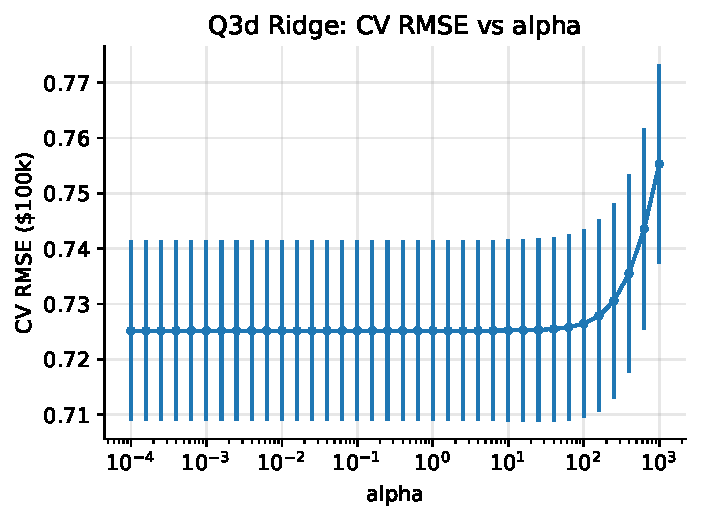
\includegraphics[width=0.45\linewidth]{figures/q3_cv_alpha_Ridge.pdf}}{}
\IfFileExists{figures/q3_cv_alpha_Lasso.pdf}{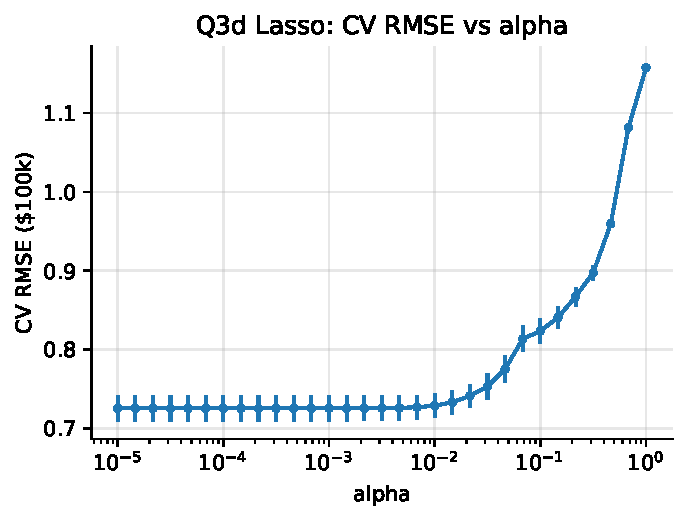
\includegraphics[width=0.45\linewidth]{figures/q3_cv_alpha_Lasso.pdf}}{}
\caption{CV RMSE vs.\ regularisation strength.}\end{figure}
\inputtable{q3_coefficients}
\inputtable{q3_sparsity}
\inputtable{q3_corr_coef_stability}

% TODO(student): interpret
\studenttodo{Q3d: shrinkage (Ridge) vs.\ sparsity (Lasso); why the CV-optimal $\alpha$ is small here (many
samples, few features); behaviour of the correlated pairs AveRooms/AveBedrms and Latitude/Longitude
(sign, magnitude, bootstrap instability).}

\fig{q3_residual_plots}{Predicted vs.\ actual and residuals vs.\ predicted on validation.}
\inputtable{q3_top_residuals}
\inputtable{q3_residual_by_band}

% TODO(student): interpret
\studenttodo{Q3e: interpret MAE/RMSE/R$^2$ in \$100k units; what the residual patterns suggest (capped
target at 5.0 $\Rightarrow$ systematic under-prediction; heteroscedasticity; unusual block groups such as very
high AveOccup); discuss at least five of the large residuals.}

\subsection{Q4: Decision trees, bagging, boosting}
\inputtable{q4_dt_criterion}
\inputtable{q4_dt_top10}
\inputtable{q4_dt_complexity}
\fig{q4_small_tree}{Depth-3 decision tree.}
\inputtable{q4_decision_paths}

% TODO(student): interpret
\studenttodo{Q4b: Gini vs.\ entropy (and log\_loss = entropy in sklearn, see \texttt{results/q4\_logloss\_check.json});
effect of each complexity control; interpret at least three decision paths in domain terms.}

\fig{q4_rf_curves}{Random Forest: training vs.\ validation Macro-F1.}
\inputtable{q4_rf_cv_results}
\inputtable{q4_rf_tree_correlation}
\fig[0.6]{q4_rf_tree_correlation}{Tree correlation vs.\ max\_features.}

% TODO(student): interpret
\studenttodo{Q4c: how bagging and random feature subsets reduce variance and tree correlation; trade-off
between single-tree strength and correlation; behaviour with number of trees and depth.}

\fig{q4_boosting_staged}{Boosting: staged training/validation Macro-F1 and CV grid vs.\ number of estimators.}
\inputtable{q4_AdaBoost_cv_top}
\inputtable{q4_GradientBoosting_cv_top}

% TODO(student): interpret
\studenttodo{Q4d: learning rate vs.\ number of estimators; sequential error correction (boosting reduces bias)
vs.\ independent bagged learners (variance reduction); effect of balanced sample weights. Note that the
CV-optimal n\_estimators lies at the upper end of the grid (see the CV tables) -- discuss what this implies.}

\inputtable{q4_comparison}
\inputtable{q4_importance_rank_corr}
\inputtable{q4_importance_RandomForest}
\inputtable{q4_importance_GradientBoosting}
\fig{q4_importances}{Built-in impurity importance vs.\ permutation importance on validation.}
\inputtable{q4_importance_control}
\fig{q4_importance_control}{Importance control experiment with added noise and near-duplicate features.}

% TODO(student): interpret
\studenttodo{Q4e: compare Macro-F1, accuracy, training and inference time; agreement between built-in and
permutation importance; at least two cases where importance misleads (impurity bias towards
high-cardinality/continuous features, importance split between correlated/duplicate features, importance
computed on training data, importance $\neq$ causality).}

\section{Error analysis, robustness, uncertainty, and limitations}
\label{sec:errors}

\subsection{Q2e: Validation error analysis}
The finalised Q2 candidate (best CV Macro-F1, see \texttt{results/models/q2\_best.json}) was analysed on
validation only. All misclassified validation rows are in \texttt{results/tables/q2\_errors\_all.csv}.
\inputtable{q2_errors}
\inputtable{q2_error_groups}
\inputtable{q2_error_numeric_profile}

% TODO(student): interpret
\studenttodo{Q2e: categorise at least ten errors into patterns (e.g.\ confident FPs with
\texttt{poutcome}=success, FNs among first-time contacts with no history, seasonal months, \texttt{contact}
missing); connect them to input characteristics; propose concrete improvements (features, representation,
threshold, model class) without using test labels.}

\subsection{Q5a: Cross-validation variability}
\inputtable{q5_repeated_cv}
\fig[0.85]{q5_repeated_cv_box}{Fold-wise Macro-F1 of frozen candidates.}

\subsection{Q5b: Robustness}
\inputtable{q5_robustness}
\inputtable{q5_robustness_retention}
\fig{q5_robustness}{Validation Macro-F1 vs.\ corruption severity (mean $\pm$ SD over 5 repetitions).}

% TODO(student): interpret
\studenttodo{Q5a/b: which models are stable across folds; which degrade fastest under noise/missingness and
why (distance-based kNN vs.\ trees' thresholds vs.\ linear models; how imputation interacts with missingness).
Is the scenario realistic for this domain?}

\subsection{Q5c: Paired bootstrap}
\inputtable{q5_bootstrap}
\fig[0.7]{q5_bootstrap}{Bootstrap distribution of the Macro-F1 difference.}

% TODO(student): interpret
\studenttodo{Q5c: what the interval permits (uncertainty of the difference on this validation distribution;
whether 0 is excluded) and does not permit (no causal/general claim, does not cover training randomness or
other datasets, not a test-set statement, multiple comparisons). State sampling unit and $B$.}

\subsection{Limitations and threats to validity}
% TODO(student): interpret
\studenttodo{Threats to validity of the full study: single dataset per task, campaign data from 2008--2010
(temporal shift), no temporal split, subjective interpretability/implementation scores and weights, limited
grids, validation reused for several analyses, Macro-F1 at a fixed 0.5 threshold, etc.}

\section{Final model-selection rationale and test-set evaluation}
\label{sec:final}

\subsection{Q5d: Multi-criteria selection}
Criteria (direction): performance = repeated-CV mean Macro-F1 ($\uparrow$); stability = repeated-CV SD
($\downarrow$); robustness = absolute validation Macro-F1 at the highest Gaussian-noise severity
($\sigma = 1.0$) ($\uparrow$); interpretability and implementation simplicity = ordinal 1--5 scores set in
\texttt{src/config.py} ($\uparrow$); training cost = fit time on the training partition ($\downarrow$);
inference cost = prediction time per 1000 rows ($\downarrow$). The two cost criteria are $\log_{10}$-transformed
before normalisation. Each criterion is then min-max normalised over the candidates so that 1 = best. The
normalised areas under both degradation curves are reported alongside (Table~\ref{tab:q5_robustness_criteria})
but are not used in the weighted score. Sensitivity analysis: fixed alternative schemes, leave-one-criterion-out,
and 5{,}000 Dirichlet weight vectors drawn (i) uniformly over the simplex ($\alpha = 1$) and (ii) centred on
the base weights ($\alpha = 20\,w$).
\inputtable{q5_robustness_criteria}
\inputtable{q5_cost}
\inputtable{q5_mcda_weights}
\inputtable{q5_mcda}
\inputtable{q5_sensitivity_schemes}
\inputtable{q5_dirichlet_wins}
\fig{q5_sensitivity_heatmap}{Model ranks under alternative weighting schemes.}

Our base MCDA weights reflect realistic retail-banking deployment priorities: predictive performance receives the largest share (0.40) to drive campaign ROI, followed by corruption robustness (0.20) to handle noisy CRM records, interpretability (0.15) to satisfy regulatory auditing and explain targeting decisions to campaign managers, CV stability (0.10) for operational reliability, and training cost, inference cost, and implementation simplicity (0.05 each). Naive Bayes receives a 4/5 interpretability score (vs.\ 2/5 for RF) because every prediction decomposes directly into additive log-odds contributions per feature, whereas RF requires post-hoc approximations (e.g., SHAP) across hundreds of deep trees. Under the base scheme, Naive Bayes ranks first (0.767), ahead of Random Forest (0.726) and Decision Tree (0.652). Sensitivity analysis shows that NB wins under base, equal, robustness-heavy, and cost-heavy weights as well as six of seven leave-one-criterion-out variants; however, RF takes first place under performance-heavy (0.60), performance-only, and \emph{base without interpretability} schemes (while DT wins under interpretability-heavy). In 5,000 centered Dirichlet weight perturbations ($\alpha = 20w$), NB wins 63.3\% of draws versus 32.8\% for RF (64.8\% vs.\ 3.7\% under uniform Dirichlet), indicating moderate robustness with clear sensitivity to how heavily interpretability is valued over raw Macro-F1. Methodologically, min--max normalization is vulnerable to outlier compression---for instance, DT's extreme CV SD (0.023) compresses all other models near 1.0, and stretching tiny runtime differences (e.g., 3.6\,ms vs.\ 9.4\,ms per 1,000 rows) onto $[0,1]$ can overstate negligible cost gaps despite $\log_{10}$ scaling---and because robustness ($\sigma=1.0$ Macro-F1) correlates with clean performance, predictive accuracy is partially double-counted.

\subsection{Q5e: Frozen configuration and single test evaluation}
Frozen configurations and the selection rule (\texttt{results/models/selection\_rule.json}) were written by
\texttt{src/q5\_robustness\_selection.py} before \texttt{src/q5\_final\_test.py} was executed once. Candidates were
refit on training+validation and evaluated once on the test partition; the run is logged in
\texttt{results/logs/final\_test\_runs.log}.
\inputtable{q5_test_results}
\inputtable{q5_test_per_class}
\fig[0.4]{q5_test_confusion_selected}{Test confusion matrix of the selected model.}
\inputtable{q5_test_results_regression}

After freezing the selection rule and refitting all models on the combined training and validation splits (85\% of data), the locked test set ($n = 6{,}782$) was evaluated once. The selected Naive Bayes model achieves a test Macro-F1 of 0.667 (95\% CI $[0.651, 0.684]$), accuracy of 0.857, ROC-AUC of 0.763, and PR-AUC of 0.391 (TN $= 5{,}468$, FP $= 521$, FN $= 448$, TP $= 345$). Its progression across CV (0.665), validation (0.662), and test (0.667)---mirrored by RF (0.697 $\to$ 0.706 $\to$ 0.704) and GB (0.664 $\to$ 0.674 $\to$ 0.666)---demonstrates near-zero generalization gap and validates the leakage-free protocol. Consistent with validation, Random Forest leads in raw test Macro-F1 at 0.704 ($[0.687, 0.720]$), with non-overlapping confidence intervals relative to NB; nevertheless, switching to RF after observing test outcomes would constitute test-set leakage and violate pre-registered MCDA selection, since NB was deliberately chosen for its multi-criteria balance rather than peak Macro-F1 alone. Decision Tree scores notably higher on validation (0.696) and test (0.699) than its CV mean (0.664), reflecting both its high fold-to-fold variance (SD $= 0.023$) and the benefit of refitting on 15\% additional data. Similarly, in the California Housing test evaluation, refitting on train+val helps lift test $R^2$ slightly above validation across all models (e.g., RF $0.807 \to 0.826$, DT $0.700 \to 0.742$, OLS $0.587 \to 0.604$), though all earlier dataset and protocol limitations remain applicable.

\section{LLM Usage Disclosure}
\label{sec:llm}

Large language model tools were used strictly for permitted engineering and workflow-support tasks, as documented in \texttt{LLM\_USAGE\_LOG.md}. Specifically, Antigravity was used to convert the assignment specification PDF into Markdown, structure the initial implementation specification (\texttt{AGENT\_PROMPT.md}), explain generated tables and figures, and review methodological completeness; a coding agent was used to implement the Python experiment scripts (\texttt{src/q1\_*.py} through \texttt{src/q5\_final\_test.py}), configure the virtual environment, debug pipeline code, and generate the result tables and plots. Follow-up prompts were limited to adjusting the MCDA criteria/weights and adding $k = 1$ to the $k$NN hyperparameter grid prior to locking the test set. While LLM suggestions were consulted when formulating the MCDA weights and interpretability ratings, all final design choices and trade-off approvals were made by the author. Every reported metric, table, and figure originates directly from executed, reproducible code under the locked protocol---no numbers or findings were fabricated---and the final scientific interpretations presented in this report have been reviewed and authored in my own words.

\section{References and reproducibility appendix}
\label{sec:repro}

\paragraph{Repository.} \RepoURL

\paragraph{Setup and commands} (Windows PowerShell; on Linux/macOS use \texttt{.venv/bin/python}):
\begin{verbatim}
python -m venv .venv
.venv\Scripts\python -m pip install -r requirements.txt
.venv\Scripts\python run_all.py --clean        # full pipeline, incl. the single test run
# individual steps
.venv\Scripts\python -m src.q1_data_leakage
.venv\Scripts\python -m src.q2_classifiers
.venv\Scripts\python -m src.q3_regression
.venv\Scripts\python -m src.q4_trees_ensembles
.venv\Scripts\python -m src.q5_robustness_selection
.venv\Scripts\python -m src.q5_final_test      # guarded: runs once (use --force to repeat; logged)
cd report; latexmk -pdf main.tex
\end{verbatim}

\paragraph{Configuration.} All seeds, paths, grids and weights: \texttt{src/config.py}. Split indices:
\texttt{data/splits/}. Frozen configurations: \texttt{results/models/final\_*.json} and
\texttt{results/models/selection\_rule.json}. Runtime per step: \texttt{results/logs/runtime.json}.

\paragraph{Software.} scikit-learn \cite{pedregosa2011scikit}, imbalanced-learn \cite{lemaitre2017imbalanced},
pandas, NumPy, Matplotlib, seaborn; SMOTE \cite{chawla2002smote}; Random Forests \cite{breiman2001random};
gradient boosting \cite{friedman2001greedy}; AdaBoost \cite{freund1997decision}.


\bibliographystyle{plain}
\bibliography{references}
\end{document}
